\documentclass{beamer}
\usepackage[utf8]{inputenc}

\usetheme{Madrid}
\usecolortheme{default}
\usepackage{amsmath,amssymb,amsfonts,amsthm}
\usepackage{txfonts}
\usepackage{tkz-euclide}
\usepackage{listings}
\usepackage{adjustbox}
\usepackage{array}
\usepackage{tabularx}
\usepackage{gvv}
\usepackage{lmodern}
\usepackage{circuitikz}
\usepackage{tikz}
\usepackage{graphicx}

\setbeamertemplate{page number in head/foot}[totalframenumber]

\usepackage{tcolorbox}
\tcbuselibrary{minted,breakable,xparse,skins}



\definecolor{bg}{gray}{0.95}
\DeclareTCBListing{mintedbox}{O{}m!O{}}{%
	breakable=true,
	listing engine=minted,
	listing only,
	minted language=#2,
	minted style=default,
	minted options={%
		linenos,
		gobble=0,
		breaklines=true,
		breakafter=,,
		fontsize=\small,
		numbersep=8pt,
		#1},
	boxsep=0pt,
	left skip=0pt,
	right skip=0pt,
	left=25pt,
	right=0pt,
	top=3pt,
	bottom=3pt,
	arc=5pt,
	leftrule=0pt,
	rightrule=0pt,
	bottomrule=2pt,
	toprule=2pt,
	colback=bg,
	colframe=orange!70,
	enhanced,
	overlay={%
		\begin{tcbclipinterior}
			\fill[orange!20!white] (frame.south west) rectangle ([xshift=20pt]frame.north west);
	\end{tcbclipinterior}},
	#3,
}
\lstset{
	language=C,
	basicstyle=\ttfamily\small,
	keywordstyle=\color{blue},
	stringstyle=\color{orange},
	commentstyle=\color{green!60!black},
	numbers=left,
	numberstyle=\tiny\color{gray},
	breaklines=true,
	showstringspaces=false,
}
%------------------------------------------------------------
%This block of code defines the information to appear in the
%Title page
\title %optional
{4.3.32}

%\subtitle{A short story}

\author % (optional)
{Nipun Dasari - EE25BTECH11042}



\begin{document}
	
	\frame{\titlepage}
	\begin{frame}{Question}
		Find the coordinates of the point where the line through the points P\brak{4, 3, 2} and Q\brak{5, 1, 6} crosses the XZ plane. Also find the angle which this line makes with the XZ plane. Solve using matrices and vectors only.
	\end{frame}
	
	
	\begin{frame}{Theoretical Solution}
	First, we represent the points P and Q as position vectors.
	\begin{align}
		\vec{p} = \myvec{4 \\ 3 \\ 2}  \text{and}  \vec{q} = \myvec{5 \\ 1 \\ 6}
	\end{align}
	The direction vector, $\vec{d}$
	\begin{align}
		\vec{d} = \vec{q} - \vec{p} = \myvec{5 \\ 1 \\ 6} - \myvec{4 \\ 3 \\ 2} = \myvec{1 \\ -2 \\ 4}
	\end{align}
	Line can be written as $\vec{r} = \vec{p} + \lambda \vec{d}$.
	\begin{align}
		\vec{r} = \myvec{x \\ y \\ z} = \myvec{4 \\ 3 \\ 2} + \lambda \myvec{1 \\ -2 \\ 4} = \myvec{4 + \lambda \\ 3 - 2\lambda \\ 2 + 4\lambda}
	\end{align}
	The line crosses the XZ plane where the y-coordinate is 0.
	\begin{align}
		3 - 2\lambda = 0 \implies 2\lambda = 3 \implies \lambda = \frac{3}{2} \label{0.4}
	\end{align}
	
	\end{frame}
	\begin{frame}{Theoretical Solution}
	The line crosses the XZ plane where the y-coordinate is 0.
	\begin{align}
		3 - 2\lambda = 0 \implies 2\lambda = 3 \implies \lambda = \frac{3}{2} \label{0.4}
	\end{align}
	By \eqref{0.4}
	\begin{align}
		\vec{r}_{\text{intersection}} = \myvec{4 + \frac{3}{2} \\ 3 - 2(\frac{3}{2}) \\ 2 + 4(\frac{3}{2})} = \myvec{\frac{11}{2} \\ 0 \\ 8}
	\end{align}
	The intersection point is $(\frac{11}{2}, 0, 8)$.
	
	The angle $\theta$ between a line with direction vector $\vec{d}$ and a plane with normal vector $\vec{n}$ is given by:
	\begin{align}
		\cos\brak{\pi/2-\theta}= \frac{|\vec{d}^T\vec{n}|}{\norm{\vec{d}} \norm{\vec{n}}} \label{0.6}
	\end{align}
	The direction vector of the line is $\vec{d} = \myvec{1 \\ -2 \\ 4}$. The normal vector to the XZ plane ($y=0$) is $\vec{n} = \myvec{0 \\ 1 \\ 0}$.
	\end{frame}

\begin{frame}{Theoretical Solution}
\begin{align}
	\vec{d}^T\vec{n} = \myvec{1 \\ -2 \\ 4}^T\myvec{0 \\ 1 \\ 0} = (1)(0) + (-2)(1) + (4)(0) = -2 \label{0.7}
\end{align}

\begin{align}
	\norm{\vec{d}} = \sqrt{1^2 + (-2)^2 + 4^2} = \sqrt{1 + 4 + 16} = \sqrt{21} \label{0.8} \\ 
	\norm{\vec{n}} = \sqrt{0^2 + 1^2 + 0^2} = 1 \label{0.9}
\end{align}
By \eqref{0.6},\eqref{0.7},\eqref{0.8},\eqref{0.9}
\begin{align}
	\sin\theta = \frac{-2}{\sqrt{21}1} = \frac{-2}{\sqrt{21}}
\end{align}
Therefore, the angle the line makes with the XZ plane is:
\begin{align}
	\theta = \arcsin\brak{\frac{-2}{\sqrt{21}}}
\end{align}
\end{frame}
	\begin{frame}[fragile]
		\frametitle{C Code- Triangle Area function }
		
		\begin{lstlisting}
			#include <stdio.h>
			void calculate_plot_data(const double* p, const double* q,
			double* intersection_point,
			double* line_segment_x,
			double* line_segment_y,
			double* line_segment_z,
			int num_line_points) {
				// Direction vector d = q - p
				double d[3];
				d[0] = q[0] - p[0]; // dx
				d[1] = q[1] - p[1]; // dy
				d[2] = q[2] - p[2]; // dz
		\end{lstlisting}
	\end{frame}
	\begin{frame}[fragile]
		\frametitle{C Code- Triangle Area function }
		
		\begin{lstlisting}
		 // Find lambda for intersection with the XZ plane (where y=0)
		// y(lambda) = p[1] + lambda * d[1] = 0  =>  lambda = -p[1] / d[1]
		double lambda_intersect = -p[1] / d[1];
		
		// Calculate and store the intersection point
		intersection_point[0] = p[0] + lambda_intersect * d[0];
		intersection_point[1] = 0.0; // By definition of the XZ plane
		intersection_point[2] = p[2] + lambda_intersect * d[2];
		
			\end{lstlisting}
		\end{frame}
		\begin{frame}[fragile]
			\frametitle{C Code- Triangle Area function }
			
			\begin{lstlisting}
				// Define a range for the parameter lambda to plot a nice segment of the line
				double lambda_start = -1.0;
				double lambda_end = 2.5;
				double lambda_step = (lambda_end - lambda_start) / (num_line_points - 1);
				
				// Generate points for the line segment
				for (int i = 0; i < num_line_points; ++i) {
					double lambda = lambda_start + i * lambda_step;
					line_segment_x[i] = p[0] + lambda * d[0];
					line_segment_y[i] = p[1] + lambda * d[1];
					line_segment_z[i] = p[2] + lambda * d[2];
				}
				
				\end{lstlisting}
			\end{frame}
	
	\begin{frame}[fragile]
		\frametitle{Python Code using shared output}
		\begin{lstlisting}
			import ctypes
			import numpy as np
			import matplotlib.pyplot as plt
			from mpl_toolkits.mplot3d import Axes3D
			import os
			# --- Step 1: Load the compiled shared library ---
			lib = ctypes.CDLL("./4.11.19.so")
			# --- Step 2: Define the function signature (argument and return types) ---
			lib.calculate_plot_data.argtypes = [
			np.ctypeslib.ndpointer(dtype=np.float64, ndim=1, flags='C_CONTIGUOUS'), # p
			np.ctypeslib.ndpointer(dtype=np.float64, ndim=1, flags='C_CONTIGUOUS'), # q
			np.ctypeslib.ndpointer(dtype=np.float64, ndim=1, flags='C_CONTIGUOUS'), # intersection_point (output)
			np.ctypeslib.ndpointer(dtype=np.float64, ndim=1, flags='C_CONTIGUOUS'), # line_x (output)
			np.ctypeslib.ndpointer(dtype=np.float64, ndim=1, flags='C_CONTIGUOUS'), # line_y (output)
			np.ctypeslib.ndpointer(dtype=np.float64, ndim=1, flags='C_CONTIGUOUS'), # line_z (output)
			ctypes.c_int  # num_line_points
			]
			lib.calculate_plot_data.restype = None
		\end{lstlisting}
	\end{frame}
	\begin{frame}[fragile]
		\frametitle{Python Code using shared output}
		\begin{lstlisting}		
		# --- Step 3: Prepare data and call the C function ---
		p_point = np.array([4, 3, 2], dtype=np.float64)
		q_point = np.array([5, 1, 6], dtype=np.float64)
		
		# Allocate memory for the output arrays that the C function will modify
		num_line_points = 100
		intersection_point = np.zeros(3, dtype=np.float64)
		line_x = np.zeros(num_line_points, dtype=np.float64)
		line_y = np.zeros(num_line_points, dtype=np.float64)
		line_z = np.zeros(num_line_points, dtype=np.float64)
		
		# Execute the function from our .so library
		lib.calculate_plot_data(
		p_point, q_point, intersection_point,
		line_x, line_y, line_z, num_line_points
		)
		
		print(f"Intersection point from C library: {intersection_point}")
			
		\end{lstlisting}
	\end{frame}
	\begin{frame}[fragile]
		\frametitle{Python Code using shared output}
		\begin{lstlisting}
		# --- Step 4: Create the 3D plot with Matplotlib ---
		fig = plt.figure(figsize=(10, 8))
		ax = fig.add_subplot(111, projection='3d')
		
		# Plot the XZ plane surface
		plane_x_range = np.arange(2, 9, 1)
		plane_z_range = np.arange(0, 13, 1)
		plane_xx, plane_zz = np.meshgrid(plane_x_range, plane_z_range)
		plane_yy = np.zeros_like(plane_xx)
		ax.plot_surface(plane_xx, plane_yy, plane_zz, alpha=0.2, color='c', rstride=10, cstride=10)
		
		# Plot the line calculated by the C function
		ax.plot(line_x, line_y, line_z, color='m', label='Line through P and Q')
		\end{lstlisting}
	\end{frame}
	\begin{frame}[fragile]
		\frametitle{Python Code using shared output}
		\begin{lstlisting}
			# Plot the points
			ax.scatter(*p_point, color='blue', s=100, label=f'P {tuple(p_point)}')
			ax.scatter(*q_point, color='green', s=100, label=f'Q {tuple(q_point)}')
			ax.scatter(*intersection_point, color='red', s=150, zorder=10, marker='*', label=f'Intersection')
			
			# Formatting the plot
			ax.set_xlabel('X-axis'), ax.set_ylabel('Y-axis'), ax.set_zlabel('Z-axis')
			ax.set_title('Line Intersection with XZ Plane')
			ax.legend()
			ax.view_init(elev=20, azim=-60)
			plt.show()
		\end{lstlisting}
	\end{frame}
	
	
	
	\begin{frame}{Plot by python using shared output from c}
		\begin{center}
			\begin{figure}[H]
				\centering
				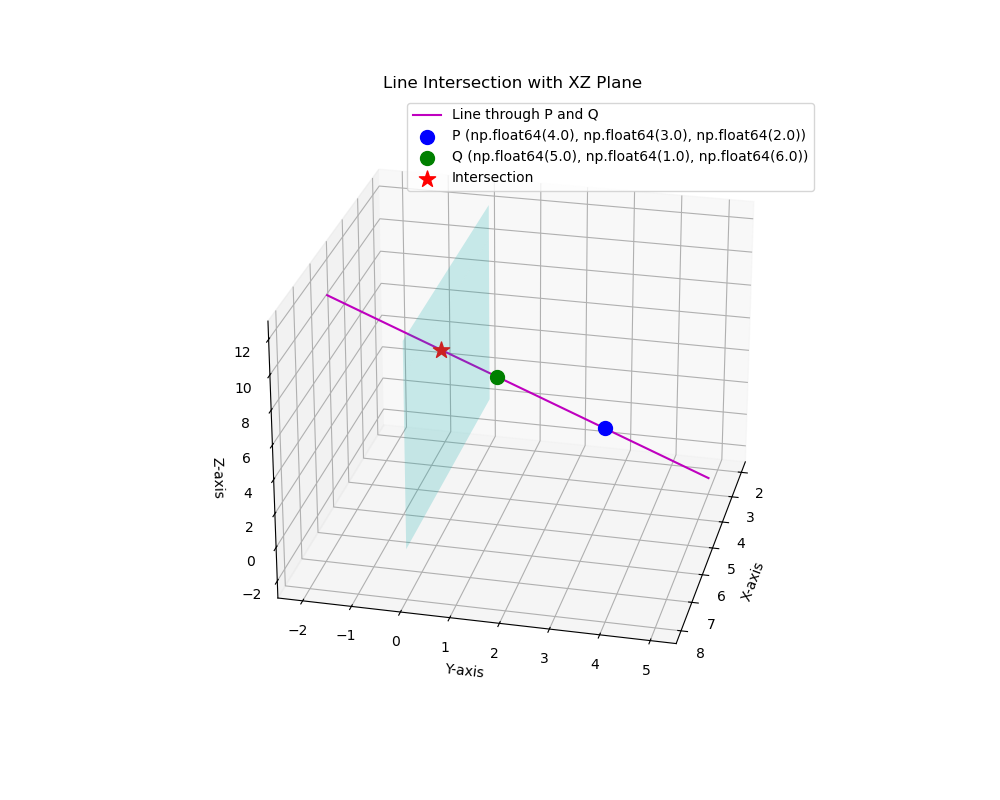
\includegraphics[width = 0.8\columnwidth]{figs/Figure_1.png}
				\caption*{}
				\label{}
			\end{figure}
		\end{center}
	\end{frame}
	
	
\end{document}